\section{Lecture 5: Spike-Train Decoding and Information}
\label{sec:aand-spikes-lecture-5}

Lecture 4 asked how a time-dependent stimulus can predict a time-dependent firing rate. Lecture 5 turns the arrow around. The data analyst now observes spikes and asks what those spikes allow one to infer about the stimulus. This is the decoding problem:
\[
    s(t) \longleftarrow \rho(t).
\]

The lecture has two connected parts. The first part derives a linear spike-train decoder and shows why a prediction delay is unavoidable for causal decoding. The second part introduces entropy and mutual information as a way to quantify how much a neural response says about a stimulus, independent of a particular decoder.

\subsection{From recorded spike events to variables one can decode from}

The practical problem is that the recording system gives discrete events, while the scientific question is usually about a continuous stimulus, movement, or internal state. The mental model is a measurement pipeline: raw voltage is reduced to spike times, spike times are organized into response summaries, and those summaries are then used either to estimate a stimulus or to measure information about it.

\subsubsection{The retained measurements}

The canonical starting point is still the spike train
\[
    \rho(t)=\sum_{i=1}^{n}\delta(t-t_i),
\]
where each $t_i$ is the time of one detected spike in an observation window. The object $\rho(t)$ is a point-process representation: it does not preserve the exact extracellular waveform, but it preserves the event times used by rate estimation, correlation analysis, decoding, and likelihood models.

For Lecture 5, the important response summaries are the following.

\paragraph{Raster plots.}
A raster arranges spike times by trial. Its role is diagnostic: it shows whether spikes are stimulus locked, whether different trials have comparable timing, and whether one should trust a trial-averaged summary. A raster is not itself a model; it is the quickest way to see whether the model assumptions are plausible.

\paragraph{Spike-count windows.}
For a window $[a,b]$, the count
\[
    N_{[a,b]}=\int_a^b \rho(t)\,d t
\]
is the number of spikes retained from that interval. Varying the window changes the response variable. A short window keeps timing but has high variability; a long window stabilizes the count but discards temporal structure.

\paragraph{Firing-rate and PSTH estimates.}
If trial $k$ contributes $n_{kj}$ spikes to bin $j$ of width $\Delta t$, a peristimulus time histogram estimates
\[
    \widehat r_j
    =
    \frac{1}{N_{\mathrm{trials}}\Delta t}
    \sum_{k=1}^{N_{\mathrm{trials}}} n_{kj}.
\]
The numerator adds spike counts across repeated presentations of the same stimulus. The denominator converts that count into spikes per unit time per trial. The result is a stimulus-locked average rate, useful when a decoder or information calculation needs a repeatable response summary rather than a single noisy spike train.

\paragraph{Interspike intervals, variability, and refractory checks.}
The intervals
\[
    \Delta_i=t_{i+1}-t_i
\]
measure the local spacing between spikes. Their coefficient of variation,
\[
    \mathrm{CV}_{\mathrm{ISI}}
    =
    \frac{\mathrm{std}(\Delta_i)}{\mathrm{mean}(\Delta_i)},
\]
compares interval variability to the mean interval. Refractory effects appear as a shortage of very small $\Delta_i$ values. Spike-count variability is often summarized by the Fano factor
\[
    F_\Delta
    =
    \frac{\mathrm{Var}(N_\Delta)}{\mathbb{E}[N_\Delta]},
\]
where $N_\Delta$ is the spike count in a fixed window. For a homogeneous Poisson process, $F_\Delta=1$ and $\mathrm{CV}_{\mathrm{ISI}}=1$. Deviations from those values are not nuisances; they are residual checks telling us whether a simple independent-spiking baseline is adequate.

\begin{figure}[h]
\centering
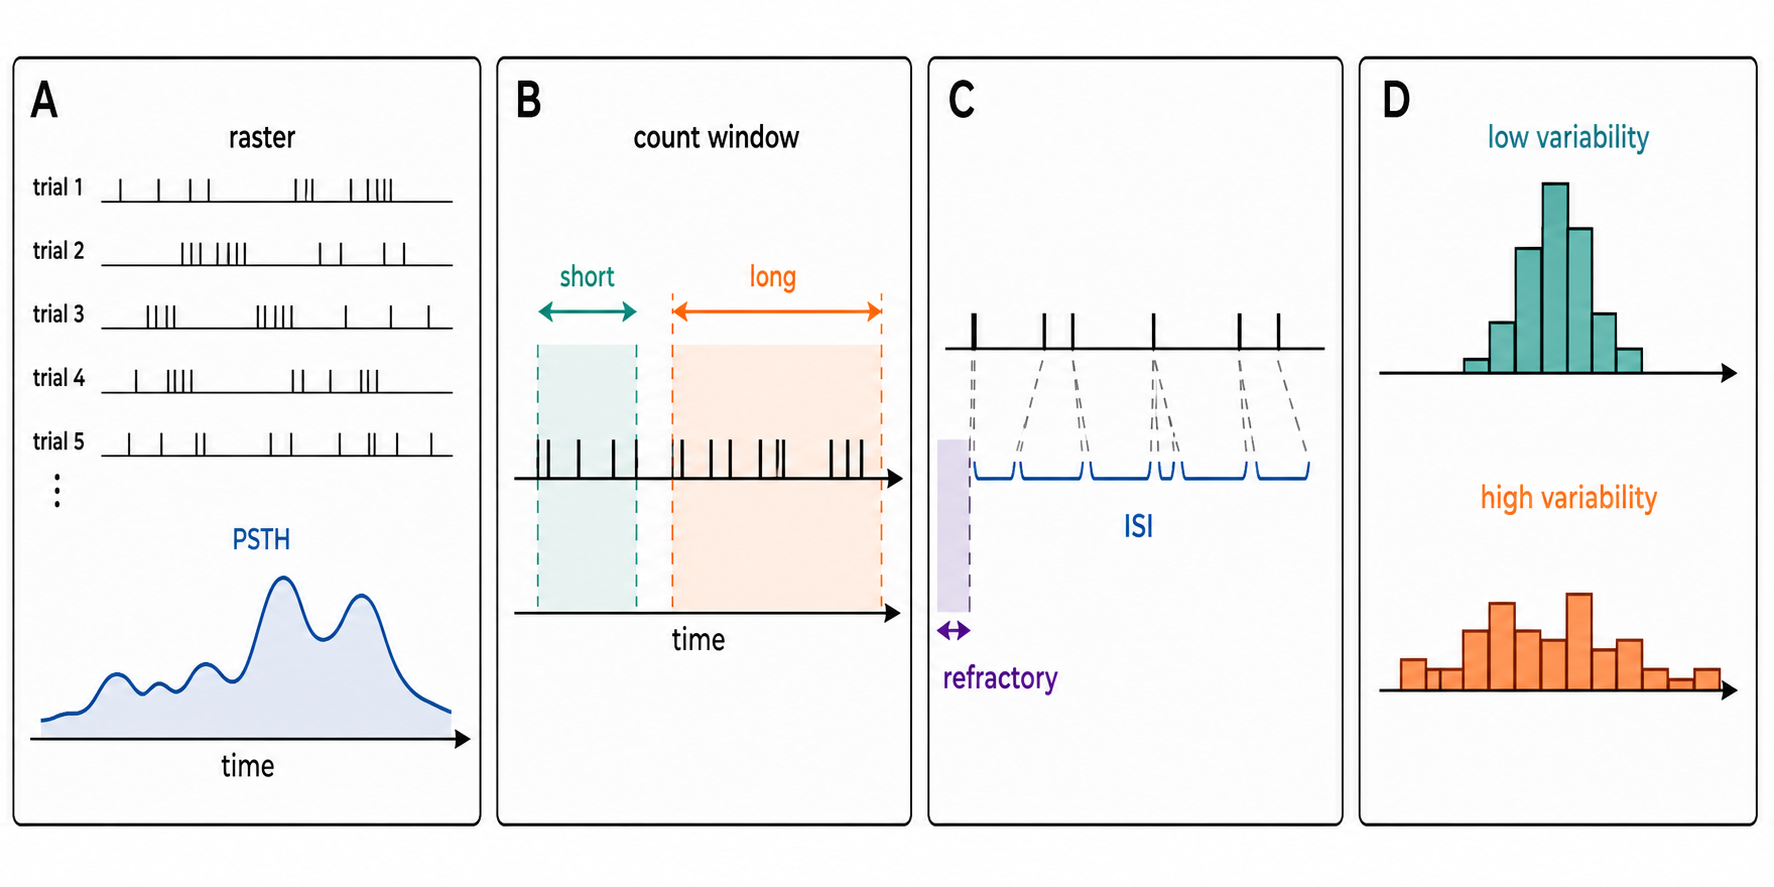
\includegraphics[width=\textwidth]{figures/aand-lecture5-spike-measurements.png}
\caption{Spike-data summaries used before decoding or information analysis. A raster and PSTH show trial-locked structure, count windows define the retained response variable, ISIs expose refractory and interval structure, and count variability checks whether repeated windows are close to a simple Poisson baseline.}
\end{figure}

\paragraph{Practical implication.}
Before decoding or computing information, decide which response variable is being retained: exact spike times, counts in windows, a PSTH, interval statistics, or a population vector. Then check spike sorting, trial alignment, stationarity, refractory violations, and bin-width sensitivity. These checks determine whether later equations are measuring neural structure or artifacts of acquisition and preprocessing.

\subsection{Why causal decoding needs a delay}

The problem solved by the decoding delay is temporal causality. At time $t$, one cannot use spikes that have not yet happened. More subtly, a spike at time $t_i$ is caused by stimulus history before $t_i$, not by a future white-noise stimulus value after $t_i$. Therefore an online decoder cannot honestly estimate the stimulus at the current time from current and past spikes unless it waits.

The lecture's mental model is a sliding causal window. At clock time $t$, the decoder estimates the earlier stimulus value $s(t-\tau_0)$, where $\tau_0$ is the prediction delay. The spikes available to the decoder are those with $t_i<t$. Among those, the most directly relevant spikes are the ones that could have been influenced by $s(t-\tau_0)$ through the stimulus-response filter.

\begin{figure}[h]
\centering
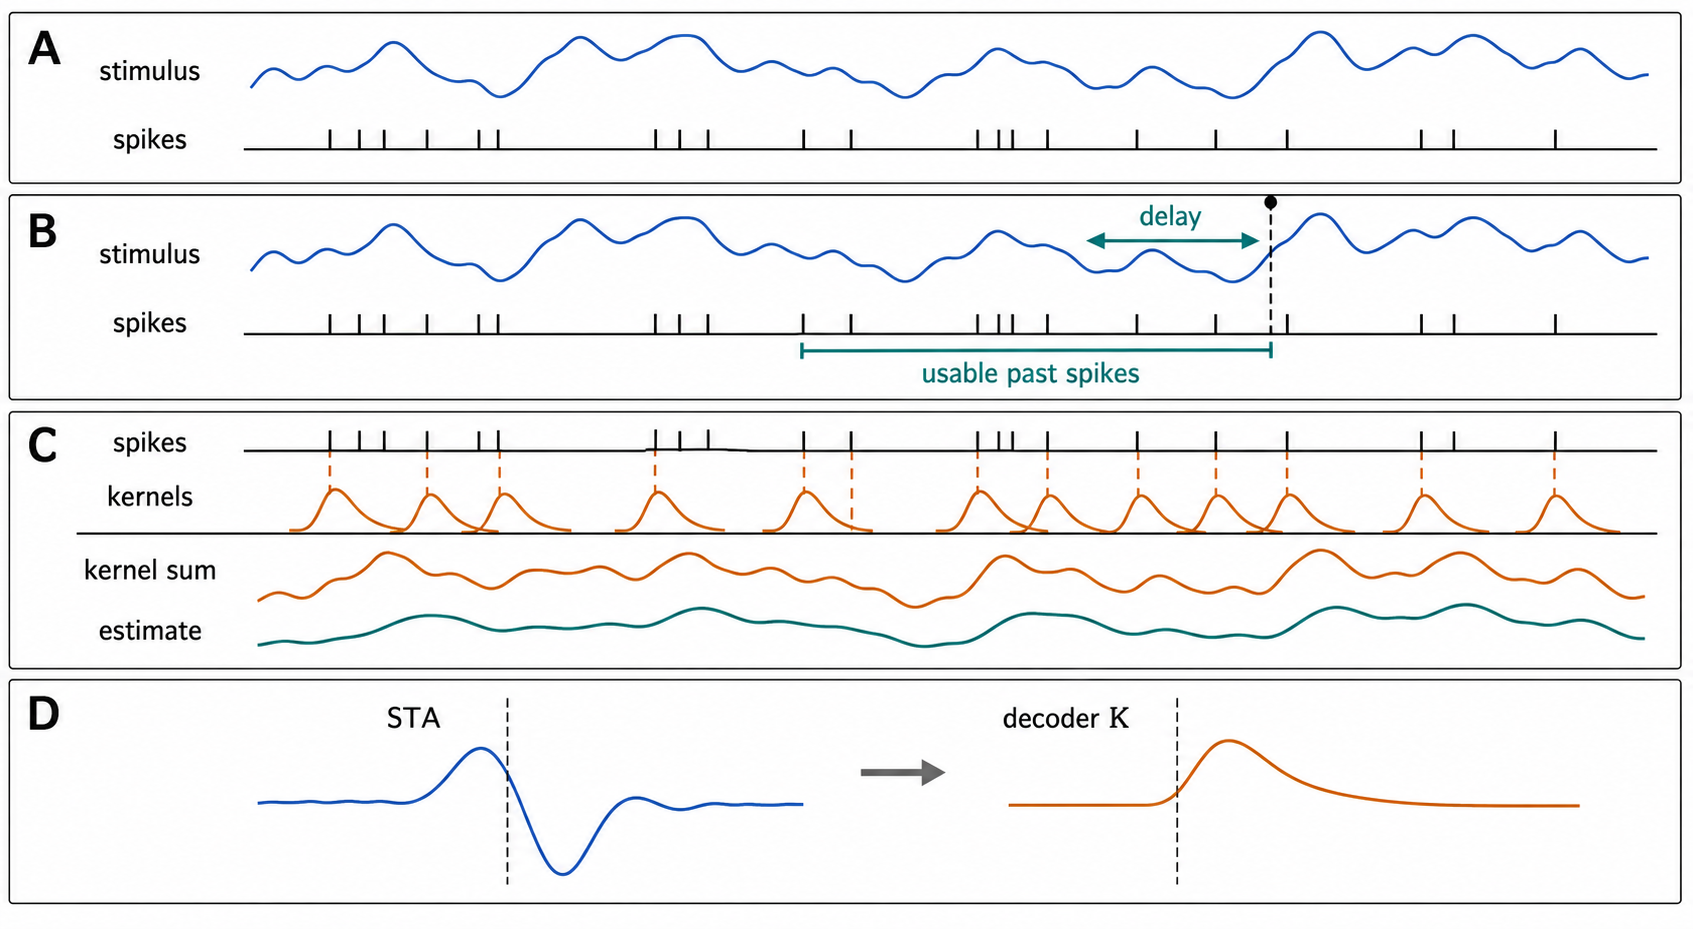
\includegraphics[width=\textwidth]{figures/aand-lecture5-decoding-workflow.png}
\caption{Causal spike-train decoding. Discrete spike events are aligned with a decoding kernel and summed to estimate a delayed stimulus value. The delay is not cosmetic: it is the price of using only spikes that have already occurred.}
\end{figure}

\subsubsection{The scale of the delay}

If the average firing rate is $\langle r\rangle$, then the expected number of spikes in a window of length $\tau_0$ is approximately
\[
    \mathbb{E}[N_{\tau_0}] \approx \langle r\rangle \tau_0.
\]
To have at least one spike on average in the decoding window, one needs roughly
\[
    \tau_0 > \frac{1}{\langle r\rangle}.
\]
The left side is a time delay. The right side is the mean interspike interval under a constant-rate approximation. The dimensional check is useful: $\langle r\rangle$ has units spikes per second, so $1/\langle r\rangle$ has units seconds per spike.

This is only a lower-bound intuition, not a theorem that one spike is enough. A reliable decoder may require a longer delay if firing is sparse, if spike timing is noisy, or if the stimulus feature to be decoded influences spikes only after a broad temporal filter.

\paragraph{Practical implication.}
When online decoding performs poorly at short latency, ask first whether the spike train contains enough causal evidence in that window. A latency constraint is also a data constraint.

\subsection{A linear decoder for a spike train}

The problem is now to convert the available point events into a continuous estimate of the stimulus. The lecture uses the simplest ansatz: each spike contributes a shifted copy of a kernel, and the decoder adds those contributions.

\subsubsection{The spike-sum form}

Let $t_1,\dots,t_n$ be the observed spike times and let $K$ be the decoding kernel. The linear estimate is
\[
    s_{\mathrm{est}}(t-\tau_0)
    :=
    \sum_{i=1}^{n}K(t-t_i)
    -
    \langle r\rangle
    \int_{-\infty}^{+\infty}K(\tau)\,d\tau .
\]
Each term has a measurement role:
\begin{itemize}
    \item $s_{\mathrm{est}}(t-\tau_0)$ is the decoder's estimate of the stimulus at the delayed time;
    \item $\tau_0$ is the prediction delay needed for causal decoding;
    \item $K(t-t_i)$ is the contribution of spike $i$ to the estimate at clock time $t$;
    \item $\langle r\rangle=\langle n\rangle/T$ is the average firing rate;
    \item the subtractive term enforces zero mean when the stimulus has been mean-subtracted.
\end{itemize}

The expression says that decoding is a filtering operation on a point process. A spike close to the time where $K$ is large has a strong effect on the estimate; a spike where $K$ is small has little effect. Changing $K$ changes what temporal pattern of spikes counts as evidence for the stimulus.

\subsubsection{The response-function form}

Using
\[
    \rho(t)=\sum_i \delta(t-t_i),
\]
the same decoder can be written as
\[
    s_{\mathrm{est}}(t-\tau_0)
    =
    \int_{-\infty}^{+\infty}K(\tau)
    \bigl[\rho(t-\tau)-\langle r\rangle\bigr]\,d\tau .
\]
This is the decoding analogue of the encoding convolution from Lecture 4. In encoding, a stimulus filter predicted a firing rate. In decoding, a spike-train filter predicts a stimulus value. The subtraction of $\langle r\rangle$ makes the input to the kernel a fluctuation around the mean firing rate, which matches the lecture's zero-mean stimulus convention.

\subsubsection{Causality constraint on the kernel}

For an online decoder, future spikes cannot contribute. Since $K(t-t_i)$ depends on the lag from a spike to the current clock time, causal decoding requires
\[
    K(t-t_i)=0 \qquad \text{for } t-t_i<0.
\]
Equivalently, $K(\tau)$ must vanish for negative lags if $\tau$ is interpreted as elapsed time since the spike. Noncausal kernels can be useful for offline analysis, but they do not describe a real-time estimator.

\paragraph{Practical implication.}
Always label whether a decoder is online or offline. Offline reconstructions may look better because they are allowed to use future spikes.

\subsection{Estimating the decoding kernel}

The problem solved by kernel estimation is projection. Among all linear filters $K$, choose the one whose decoded stimulus is closest, on average, to the true stimulus.

\subsubsection{Mean-squared decoding error}

The lecture defines the error objective
\[
    E
    =
    \frac{1}{T}\int_0^T
    \left\langle
    \bigl[
      s_{\mathrm{est}}(t-\tau_0)-s(t-\tau_0)
    \bigr]^2
    \right\rangle
    d t .
\]
The integral averages over time, and the angle brackets average over trials or repeated stimulus-response samples. The squared term penalizes a mismatch between the reconstructed delayed stimulus and the actual delayed stimulus. Minimizing $E$ gives the best linear decoder in the mean-square sense.

Variational calculus gives the integral equation
\[
    \int_{-\infty}^{+\infty}
    Q_{\rho\rho}(\tau-\tau')K(\tau')\,d\tau'
    =
    Q_{rs}(\tau-\tau_0).
\]
The two correlation functions have distinct roles:
\begin{itemize}
    \item $Q_{\rho\rho}$ is the spike-train autocorrelation, so it measures redundancy and dependence within the response itself;
    \item $Q_{rs}$ is the response-stimulus cross-correlation, so it measures which stimulus values co-vary with response fluctuations;
    \item $K$ is the unknown filter that must turn response fluctuations into a stimulus estimate.
\end{itemize}

This equation is the decoding counterpart of the Wiener equation for the encoding kernel in Lecture 4. In both cases, the optimal filter is not just a raw cross-correlation. It must account for the autocorrelation structure of the signal being filtered.

\paragraph{Sanity check.}
If the spike train has strong autocorrelation because of bursting, refractoriness, or slow state modulation, then nearby spikes are not independent pieces of evidence. The left side of the equation corrects for that redundancy. Ignoring it would overcount repeated or correlated spikes.

\paragraph{Practical implication.}
Do not estimate a decoder only by eyeballing spike-triggered averages. First ask whether response autocorrelation is close enough to the assumed baseline.

\subsection{The Poisson and white-noise simplification}

The lecture then shows how the decoding equation becomes transparent under two strong assumptions: the spike train is a homogeneous Poisson process and the stimulus ensemble is white enough for the spike-triggered average to identify the relevant temporal feature.

\subsubsection{Homogeneous Poisson response}

For a homogeneous Poisson spike train with mean rate $\langle r\rangle$, the centered spike-train autocorrelation has the idealized form
\[
    Q_{\rho\rho}(\tau)=\langle r\rangle \delta(\tau).
\]
This says that, after subtracting the mean, all nonzero lags are uncorrelated. The only remaining covariance is the instantaneous point-process variance at zero lag.

Using the Lecture 3 relation between the response-stimulus correlation and the spike-triggered average $C$,
\[
    Q_{rs}(-\tau)=\langle r\rangle C(\tau),
\]
the decoding equation reduces to
\[
    \int_{-\infty}^{+\infty}
    \langle r\rangle \delta(\tau-\tau')K(\tau')\,d\tau'
    =
    \langle r\rangle C(\tau_0-\tau).
\]
The delta function selects $K(\tau)$ on the left, and the factor $\langle r\rangle$ cancels, giving
\[
    K(\tau)=C(\tau_0-\tau).
\]

This is the clean result emphasized in the slides: under the homogeneous-Poisson simplification, the optimal linear decoding kernel is a delayed, time-reversed version of the spike-triggered average.

\subsubsection{Why this assumption is strong}

The simplicity of
\[
    K(\tau)=C(\tau_0-\tau)
\]
comes at a cost. It assumes that $\rho$ has no relevant temporal structure beyond independent Poisson variability. But earlier lectures showed many reasons this can fail: refractory periods suppress short intervals, bursting creates short-lag excess, slow excitability changes produce count variability, and population state can create shared fluctuations.

The lecture explicitly warns that this can be unreasonable in an encoding-decoding cascade where both the encoding kernel $D$ and the decoding kernel $K$ are treated as proportional to the same STA. If the response is not Poisson, the spike-train autocorrelation must be part of the decoder.

\subsubsection{Causal truncation and the delay}

For white-noise stimuli, the useful part of $K$ is confined by causality. The slides summarize the relation as follows: $K(\tau)$ is nonzero only for
\[
    0<\tau<\tau_0
\]
in the causal white-noise case. If the stimulus has long-range autocorrelations, then spikes outside this interval can still contain indirect information about the delayed stimulus, but that information comes from stimulus correlation rather than direct causality.

\paragraph{Practical implication.}
If a decoder uses very old spikes, check whether the stimulus itself is autocorrelated. Long-range decoding performance may reflect stimulus predictability rather than neural encoding of the target time.

\subsection{Example: decoding from the fly H1 neuron}

The H1 example in the slides illustrates what the equations look like in a real sensory neuron. The stimulus is motion, and the response is a spike train. Dayan and Abbott's example compares responses to $s(t)$ and to $-s(t)$ and uses decoding kernels to reconstruct the stimulus trajectory.

The schematic form shown in the lecture is
\[
    s_{\mathrm{est}}(t-40\,\mathrm{ms})
    =
    \sum_i K(t-t_i^{(+s)})
    -
    \sum_j K(t-t_j^{(-s)}).
\]
The two sums have opposite signs because the two stimulus polarities carry opposite evidence about the motion signal. The estimate is delayed by $40\,\mathrm{ms}$, matching the causal logic above: the decoder reconstructs the recent past from spikes that have already occurred.

\paragraph{Practical implication.}
The quality of a reconstruction should be compared against the actual stimulus at the delayed time, not against the instantaneous stimulus at the clock time.

\subsection{From decoding accuracy to information}

The problem solved by information theory is that a decoder is only one possible readout. Two response codes can have different decoding performance because the chosen decoder is weak, not because the neural response contains little information. Entropy and mutual information ask a more general question: how much uncertainty about one variable is removed by observing another?

\subsubsection{Response entropy}

Let $\vec{R}$ be a random response variable. In this lecture, $\vec{R}$ can be a vector of spike-count rates, binned spike counts, or any discrete response summary derived from spike trains. If the possible responses are $\vec{r}$ with probabilities $P(\vec{r})$, the entropy is
\[
    H(\vec{R})
    :=
    \sum_{\vec{r}}P(\vec{r})
    \bigl[-\log_2 P(\vec{r})\bigr].
\]
The term $-\log_2 P(\vec{r})$ is the surprise of response $\vec{r}$. Common responses have low surprise; rare responses have high surprise. Entropy is the average surprise before the response is observed, measured in bits because the logarithm uses base 2.

\begin{figure}[h]
\centering
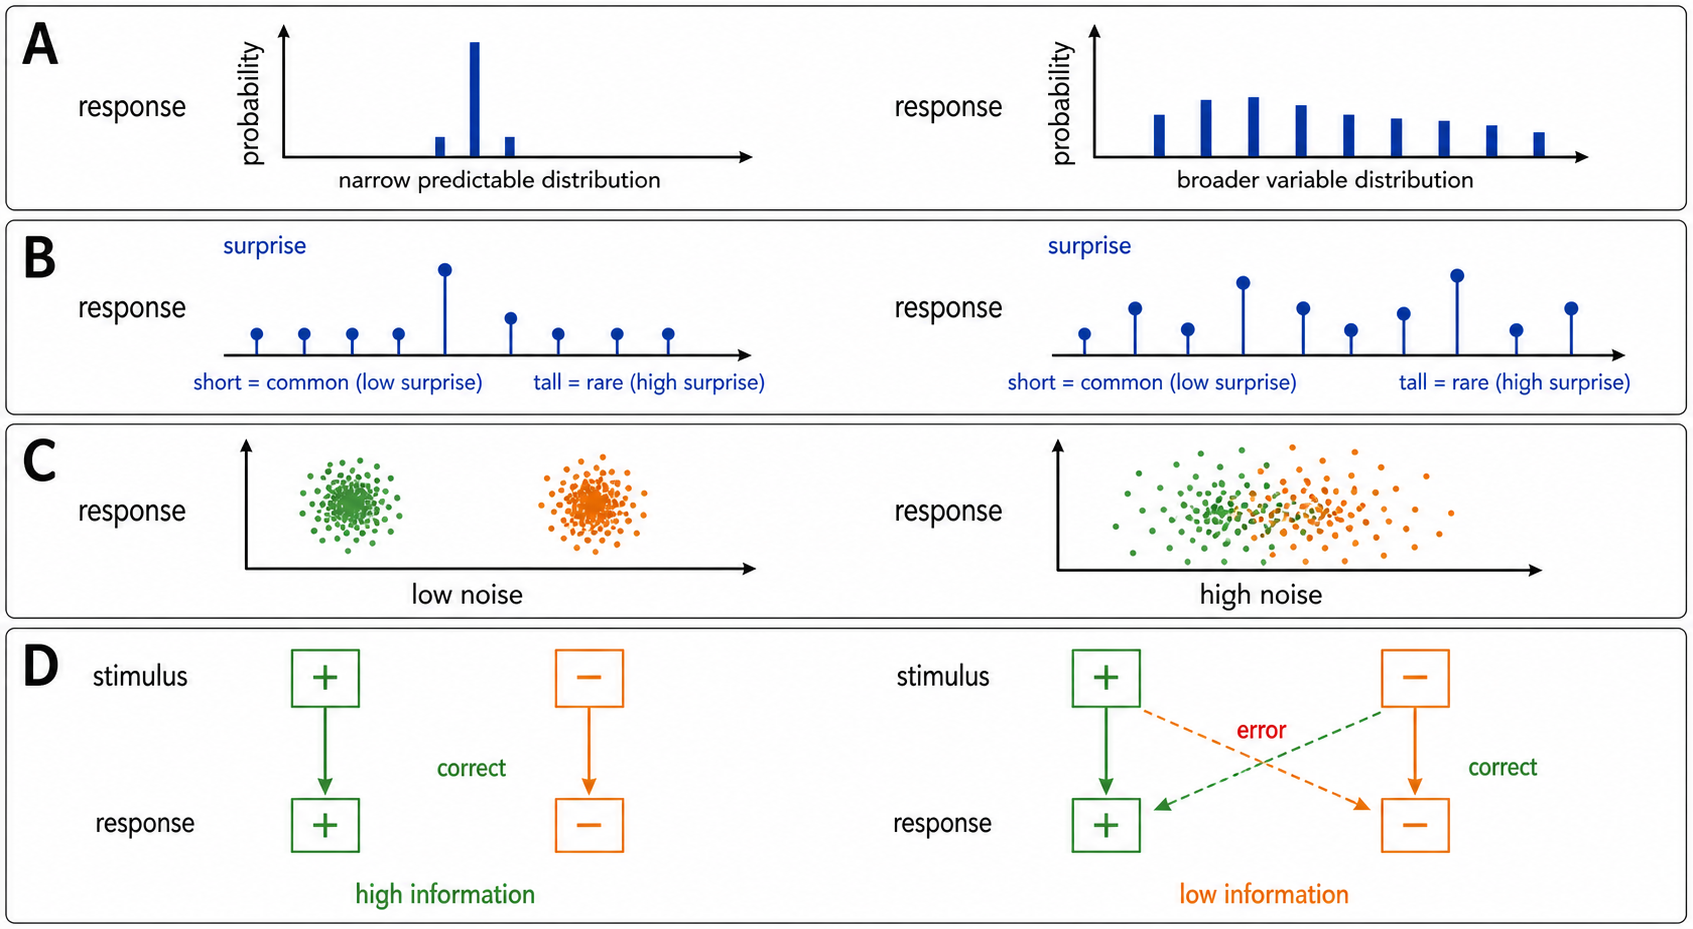
\includegraphics[width=\textwidth]{figures/aand-lecture5-information-theory.png}
\caption{Entropy and mutual information for neural responses. Broad response distributions have high entropy; rare events carry high surprise; fixed-stimulus response variability is noise entropy; and information is high when the response reduces uncertainty about the stimulus.}
\end{figure}

\paragraph{Limiting cases.}
If one response occurs with probability nearly one, then observing the response is unsurprising and $H(\vec{R})$ is near zero. If many responses occur with comparable probability, the average surprise is larger. Extremely rare events are individually surprising, but their contribution to the average entropy is small because they almost never occur.

\subsubsection{Binary response example}

For a single neuron with binary response $r\in\{r_+,r_-\}$ and
\[
    P(r_+)=p_+,\qquad P(r_-)=1-p_+,
\]
the entropy is
\[
    H(R)
    =
    p_+\bigl[-\log_2 p_+\bigr]
    +(1-p_+)\bigl[-\log_2(1-p_+)\bigr].
\]
When $p_+\to 0$ or $p_+\to 1$, the response is almost deterministic and $H(R)\to 0$. When $p_+=1/2$, both responses are equally likely and
\[
    H(R)=1\ \mathrm{bit}.
\]
The bit has a direct interpretation: one fair binary response can answer one yes-or-no question.

\subsubsection{Joint entropy and independent neurons}

For two response variables $R_1$ and $R_2$, the joint entropy is
\[
    H(R_1,R_2)
    =
    \sum_{r_1}\sum_{r_2}
    P(r_1,r_2)\bigl[-\log_2 P(r_1,r_2)\bigr].
\]
If the neurons are statistically independent,
\[
    P(r_1,r_2)=P(r_1)P(r_2),
\]
then the logarithm splits and the entropy is additive:
\[
    H(R_1,R_2)=H(R_1)+H(R_2).
\]
This is a useful benchmark. If neurons are correlated, joint entropy is not obtained by simply adding single-neuron entropies. Correlations can reduce redundant capacity or, in some regimes, create structured joint response patterns that must be modeled explicitly.

\paragraph{Practical implication.}
Before treating a population response as independent channels, compare joint variability to the product of single-neuron distributions. This is the information-theoretic version of the correlation cautions from Lectures 3 and 4.

\subsection{Mutual information between stimulus and response}

Entropy alone measures response variability, but not whether that variability is about the stimulus. A neuron can have high response entropy because it is noisy, not because it encodes much. Mutual information separates useful stimulus-related variability from noise.

\subsubsection{Definition through entropies}

For a response random variable $\vec{R}$ and stimulus random variable $S$, mutual information is
\[
    I(\vec{R},S)
    :=
    H(\vec{R})+H(S)-H(\vec{R},S).
\]
It is zero when response and stimulus are independent. It is high when observing one strongly constrains the other.

The equivalent conditional-entropy forms are
\[
    I(\vec{R},S)
    =
    H(\vec{R})-H(\vec{R}\mid S)
    =
    H(S)-H(S\mid \vec{R}).
\]
Here $H(\vec{R}\mid S)$ is the response uncertainty left when the stimulus is fixed. The lecture calls this the noise entropy:
\[
    H(\vec{R}\mid S)
    =
    \sum_s P(s)
    \left\{
    \sum_{\vec{r}}P(\vec{r}\mid s)
    \bigl[-\log_2 P(\vec{r}\mid s)\bigr]
    \right\}.
\]
The outer sum averages across stimuli. The inner sum is the entropy of responses for one fixed stimulus. If repeated presentations of the same stimulus evoke highly variable responses, the noise entropy is large and the mutual information is reduced.

\subsubsection{Definition as a divergence from independence}

The same quantity can be written as
\[
    I(\vec{R},S)
    =
    \sum_{\vec{r},s}
    P(\vec{r},s)
    \log_2
    \frac{P(\vec{r},s)}{P(\vec{r})P(s)}.
\]
This is a Kullback--Leibler divergence between the true joint distribution and the product distribution that would hold under independence. The ratio inside the logarithm asks whether a stimulus-response pair occurs more or less often than expected if response and stimulus were unrelated.

\paragraph{Deterministic and independent limits.}
If $\vec{R}$ and $S$ are independent, then $P(\vec{r},s)=P(\vec{r})P(s)$ and every logarithm is $\log_2 1=0$, so $I(\vec{R},S)=0$. If there is a unique deterministic mapping between response and stimulus, then observing the response removes all stimulus uncertainty and
\[
    I(\vec{R},S)=H(\vec{R})=H(S).
\]

\subsubsection{Binary stimulus-response channel with errors}

The slides end this part with a binary example. Let stimuli $+$ and $-$ be equally likely, so $H(S)=1$ bit. Let the response also be binary and let $P_x$ be the probability of an incorrect response:
\[
    P(r_+|-)=P(r_-|+)=P_x,\qquad
    P(r_+|+)=P(r_-|-)=1-P_x.
\]
The mutual information is
\[
    I(R,S)
    =
    1
    +(1-P_x)\log_2(1-P_x)
    +P_x\log_2 P_x.
\]
When $P_x=0$, responses are perfectly correct and $I=1$ bit. When $P_x=1/2$, the response is a fair guess and $I=0$. This example makes the role of noise entropy concrete: errors increase response uncertainty at fixed stimulus, so they reduce the stimulus information carried by the response.

\paragraph{Practical implication.}
A high firing rate or a high response entropy is not automatically a good code. The relevant question is whether response variability is aligned with stimulus variability rather than dominated by trial-to-trial noise.

\subsection{How Lecture 5 fits the course pipeline}

Lecture 5 connects the earlier spike-statistics material to inference. The pipeline is now explicit:
\begin{enumerate}
    \item acquire and sort spikes into event times;
    \item inspect rasters, rates, counts, ISIs, refractory violations, and variability to choose a response representation;
    \item estimate a decoding kernel if the goal is stimulus reconstruction;
    \item check whether the assumptions behind that kernel, especially Poisson response statistics, are defensible;
    \item use entropy and mutual information to quantify coding capacity and stimulus-related information beyond a specific decoder.
\end{enumerate}

This also foreshadows likelihood-based modeling. A decoder gives a point estimate of a stimulus. An information calculation compares distributions. A likelihood model connects the two by asking how probable the observed spikes are under a proposed stimulus-response relation. In all three cases, the analysis is only as good as the retained spike representation and the residual checks applied to it.

\subsection*{Sources mentioned in Lecture 5}

\begin{itemize}
    \item P. Dayan and L. F. Abbott (2001), \emph{Theoretical Neuroscience: Computational and Mathematical Modeling of Neural Systems}. MIT Press. Lecture 5 draws especially on Chapters 3.4 and 4.1.
    \item F. Rieke, D. Warland, R. de Ruyter van Steveninck, and W. Bialek (1997), \emph{Spikes: Exploring the Neural Code}. MIT Press, cited in the lecture slides.
\end{itemize}
